\problemname{Fabriksrobot}


\begin{figure}[ht!]
\centering
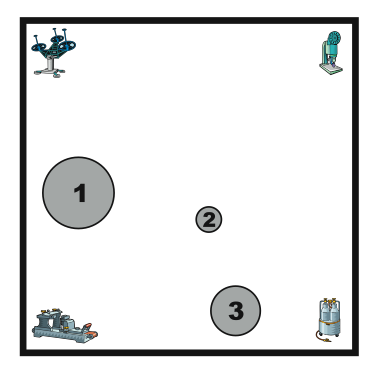
\includegraphics[width=0.7\textwidth]{fabriksrobot.png}
\caption{Förklaring till exemplet. Det kritiska avståndet är det mellan pelare 1 och 2 i indata. Avståndet mellan deras centrumpunkter är cirka 405.123, och det verkliga avståndet däremellan är 405.12 - 110 - 30 = 265.12, vilket gör att den maximala radien på roboten är 265.12/2 = 132.56.}
\label{overflow}
\end{figure}

På ett stort fabriksgolv (storlek $1000 \times 1000$ meter) finns ett antal cirkulära pelare med varierande radie. Pelarna tangerar inte varandra eller väggarna. Företaget, som äger fabriken, planerar att köpa in en vaktrobot som ska röra sig i lokalen. I lokalens fyra hörn finns maskiner placerade till vilka roboten måste kunna ta sig genom att sick-sacka fram mellan pelare och väggar. De vaktrobotar som finns på marknaden är alla, liksom pelarna, helt cirkulära. Innan företaget köper in en robot vill de dock veta vad den maximala radien på roboten får vara för att deras krav fortfarande ska kunna uppfyllas.

Ingen del av roboten får sticka ut utanför lokalen. Om roboten har radien $r$ så ska den kunna ta sig till punkterna $(r, r)$, $(1000 - r, r)$, $(r, 1000 - r)$ respektive $(1000 - r, 1000 - r)$ och därifrån betjäna de fyra maskinerna. Maskinerna utgör aldrig något hinder för robotens framfart.

\section*{Indata}
Den första raden innehåller ett heltal $n$ ($1 \le n \le 50$), antalet pelare i lokalen.

Därefter följer $n$ rader som vardera innehåller 3 heltal, $x$, $y$ och $r$. Dessa tal beskriver koordinaterna
för en pelares centrum samt dess radie.


\section*{Utdata}
Skriv ut ett flyttal: robotens maximala radie. Svaret accepteras om skillnaden mellan det och domarens
svar är mindre än $0.01$.

\section*{Poängsättning}
Din lösning kommer att testas på en mängd testfallsgrupper.
För att få poäng för en grupp så måste du klara alla testfall i gruppen.

\noindent
\begin{tabular}{| l | l | p{12cm} |}
  \hline
  \textbf{Grupp} & \textbf{Poäng} & \textbf{Gränser} \\ \hline
  $1$    & $20$       & $n = 1$ \\ \hline
  $2$    & $80$       & Inga ytterligare begränsningar. \\ \hline
\end{tabular}
